\section{RP13 Progressive Enhancement}
\label{sec:principle-rp13-progressive-enhancement}

Die Client-Technologien HTML und CSS haben sich über die Jahre weiterentwickelt. Immer aber mit dem Hintergedanke ``Progressive Enhancement''. Das bedeutet, dass die Entwicklung immer versucht hat, Rücksicht auf die älteren Browserversionen zu nehmen.
Deutlich sieht man es bei dem neuen HTML5 Standard. Neue Formulartypen wurden eingeführt wie ``tel'', ``email'', ``color'', ``date'', etc. Browser die HTML5 nicht unterstützen, weichen bei einem für sie unbekannten Typ auf einen Default zurück. Im Falle vom Formulartyp, würde es als ``text'' interpretiert werden.

\begin{lstlisting}[language=HTML, caption={Inputfeld in HTML5, welches eine Telefonnummer erwartet}, label={lst:html5TelInput}]
<input type="tel" name="telefon">
\end{lstlisting}

Natürlich gibt es keine Regel ohne Ausnahmen. Manche Tags, die im HTML5 Standard eingeführt wurden, werden überhaupt nicht beachtet. Dies kann vor allem bei Versionen kleiner als neun des Internet Explorers beobachtet werden.

\subsection*{Geplante Umsetzung}
Die Beispielanwendung soll, wie bereits in \ref{sec:requirments-engineering-nonfunctionals} erwähnt, Internet Explorer 8 und höher, Chrome 25 und höher, Firefox 19 und höher und Safari 6 und höher unterstützen.

Auch Browser auf Smartphones sollten nicht vernachlässigt werden. Hierfür sollen Safari 6 und höher und Android Browser 4.0 und höher unterstützt werden.

\subsection*{Konkrete Umsetzung}
Da alle geplanten zu unterstützenden Browser nicht HTML5 interpretieren können, musste einen kleinen Trick angewendet werden, um so die Rückwärtskompatibilität zu erhöhen. Dieser trick heisst ``modernizr'' \cite{modernizr}. Modernizr ist eine JavaScript-Bibliothek, welche gezielt den verwendeten Browser auf seine Funktions- und Unterstützungsumfang von HTML5 und CSS3 überprüft. Das Resultat wird dann in einem JavaScript-Objekt gespeichert und zur Verfügung gestellt.  Zusätzlich läuft modernizr in eine kleine Schleife, um die neuen Tag (head, section, article, nav, u.w.) zu aktivieren. Das bedeutet, dass diese Tags nicht mit ``div'' ersetzt werden müssen.

Um diese Library einzubinden, hat man nichts weiteres zu tun als das Script im Header nach dem Stylesheet hinzuzufügen.

\begin{lstlisting}[language=HTML, caption=Einbinden von modernizr \cite{roomiesLayout}, firstnumber=11, label=lst:mdernizrLayoutServer]
<link href="/stylesheets/app.css" rel="stylesheet"/>
<script src="/javascripts/lib/custom.modernizr.js"></script>
\end{lstlisting}

Mit diesem ``Trick'' konnte erreicht werden, dass in allen geplanten Browser alle Elementen erscheinen, wenn auch nicht immer korrekt. Nicht immer korrekt, weil im Internet Explorer 8, die Darstellung des Bildes im oberen linken Rand nicht dem entspricht, was erwartet wurde.

\begin{figure}[H]
	\centering
	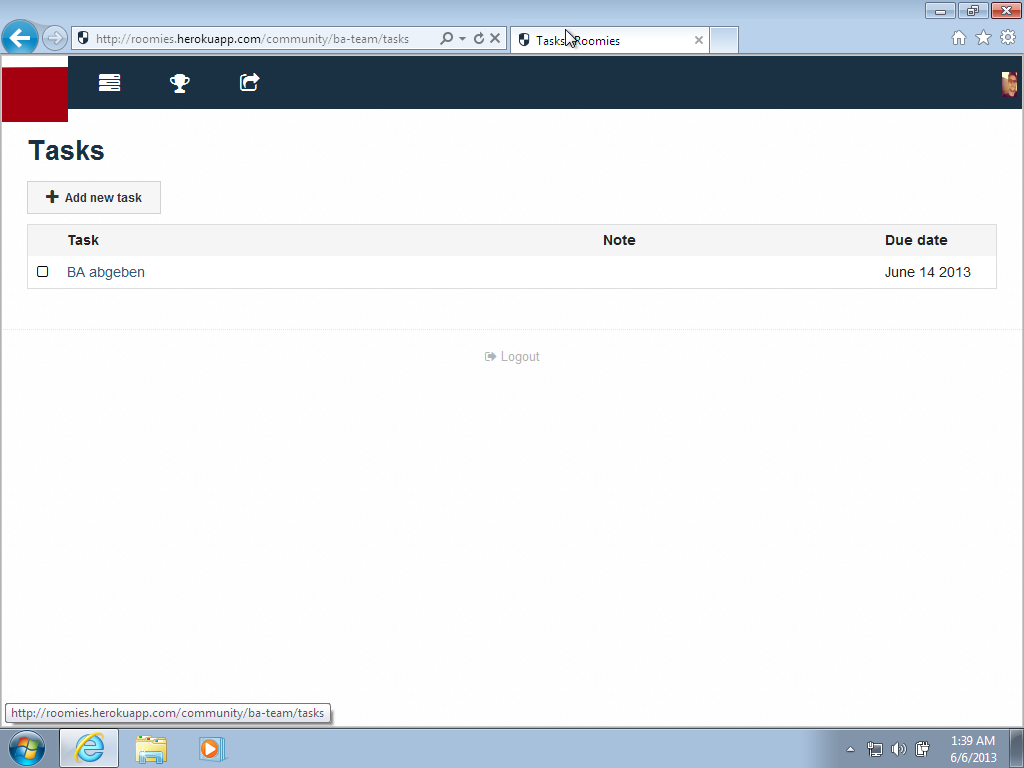
\includegraphics[width=12cm]{content/principle-demonstration/images/progressive-enhancement-ie8.png}
	\caption{Darstellung im Internet Explorer 8}
	\label{fig:iossafari-datepicker}
\end{figure}

\subsection*{Diskussion}

